\section{Casi d'Uso}\label{CasiUso}
\subsection{Introduzione}\label{CasiUso_Introduzione}
Nella seguente sezione verranno identificati i casi d'uso individuati dal team \texttt{Agents of S.W.E.}.\\
Il numero di casi analizzati è limitato poiché il plug-in fornisce funzionalità aggiuntive ad una piattaforma preesistente, per la quale non è fornita documentazione in quanto già disponibile presso il sito web del fornitore della piattaforma: \textit{Grafana Labs}\footnote{\url{http://docs.grafana.org/}}.

\subsection{Attori}\label{Attori}
E' importante notare che il numero esiguo di differenti attori che possono approcciarsi al prodotto in esame è principalmente dovuto al fatto che, essendo il progetto "G\&B" un plug-in di un sistema indipendente, poche tipologie di utenti possono effettivamente approcciarsi al prodotto finale.\\
E' altrettanto importante sottolineare che il sistema di registrazione ed autenticazione dell'utente viene gestito interamente dal sistema \textit{Grafana}, dal momento che, ovviamente, il prodotto finale non avrà una funzionalità di autenticazione interna.

\subsubsection*{Attori primari}
\begin{itemize}
\item \textbf{Utente:} Si riferisce ad un generico utente che ha effettuato l'autenticazione al sistema \textit{Grafana}. E' l'unica tipologia di utente con facoltà di interagire con il prodotto, in quanto questo risulta essere un plug-in;
\item \textbf{Piattaforma Grafana:} Sistema di monitoraggio di flusso dati, di cui il prodotto da realizzare è un plug-in. Consente agli utenti autenticati, attraverso funzionalità proprie, di realizzare grafici ed alert riferiti a dati forniti dal plug-in.
\end{itemize}

\subsubsection*{Attori secondari}
\begin{itemize}
\item \textbf{Piattaforma Grafana:} Sistema di monitoraggio di flusso dati, di cui il prodotto da realizzare è un plug-in. Consente agli utenti autenticati, attraverso funzionalità proprie, di realizzare grafici ed alert riferiti a dati forniti dal plug-in.
\end{itemize}

\subsection{Elenco dei casi d'uso}

%\begin{itemize}
%\item \textbf{Attore primario:}
%\item \textbf{Precondizioni:}
% \begin{enumerate}
% \item
% \end{enumerate}
%\item \textbf{Postcondizioni:}
% \begin{enumerate}
% \item
% \end{enumerate}
%\item \textbf{Scenario Principale:}
% \begin{enumerate}
% \item
% \end{enumerate}
%\item \textbf{Estensioni:}
%\end{itemize}

\subsubsection{UC1 - Aggiunta della rete bayesiana al plug-in G\&B}\label{UC1}

\begin{figure}[H]
	\begin{center}
		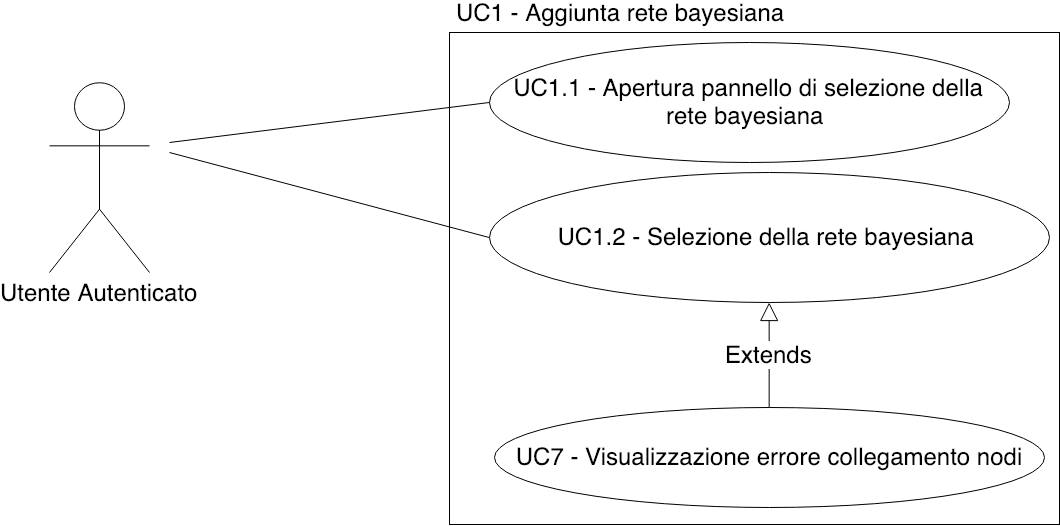
\includegraphics[scale=0.4]{./images/UC1.png}
		 \caption{UC1 - Aggiunta della rete bayesiana al plug-in G\&B}	
	\end{center}
\end{figure}
\begin{itemize}
	\item \textbf{Attore primario}: Utente;
	\item \textbf{Precondizioni}: l'utente deve aver effettuato il login nella piattaforma \textit{Grafana}, deve aver selezionato una dashboard e aggiunto il pannello "G\&B Panel";
	\item \textbf{Postcondizioni}: l'utente ha aggiunto la rete bayesiana al plug-in. Attraverso \hyperref[UC2]{UC2 (§\ref*{UC2})} può selezionare quali nodi sorgente collegare alla rete.
	\item \textbf{Scenario principale:}
	\begin{enumerate}
		\item L'utente accede alla piattaforma \textit{Grafana}, si trova nella dashboard preferita ed ha aggiunto il pannello "G\&B Panel";
		\item L'utente seleziona e clicca sul bottone con simbolo di "+"(\hyperref[UC1.1]{UC1.1 (§\ref*{UC1.1})});
		\item L'utente si trova davanti una finestra presso cui selezionare il file \textit{JSON} contenente la rete (\hyperref[UC1.2]{UC1.2 (§\ref*{UC1.2})}) e seleziona "Aggiungi".
	\end{enumerate}
	\item \textbf{Estensioni:} \hyperref[UC8]{UC8 (§\ref*{UC8})} estende \hyperref[UC1.2]{UC1.2 (§\ref*{UC1.2})}: l'utente visualizza un messaggio di errore nel caso in cui l'operazione non sia andata a buon fine.
\end{itemize}

\paragraph{UC1.1 - Apertura pannello di selezione della rete bayesiana}\label{UC1.1}
\begin{itemize}
	\item \textbf{Attore primario}: Utente; 
	\item \textbf{Precondizioni}: l'utente visualizza il pannello "G\&B Panel" nella dashboard.
	\item \textbf{Postcondizioni}: l'utente ha cliccato il bottone con etichetta "+" e visualizza il pannello per la selezione del file della rete;
	\item \textbf{Scenario principale}: l'utente seleziona clicca il pulsante con etichetta "+" nel pannello "G\&B Panel" nella dashboard.
\end{itemize}


\paragraph{UC1.2 - Selezione della rete bayesiana}\label{UC1.2}
\begin{itemize}
	\item \textbf{Attore primario}: Utente;
	\item \textbf{Precondizioni}: l'utente ha cliccato il bottone con etichetta "+";
	\item \textbf{Postcondizioni}: l'utente ha selezionato la rete bayesiana desiderata e ha premuto il pulsante con etichetta "Aggiungi";
	\item \textbf{Scenario principale}:
	\begin{enumerate}
		\item L'utente seleziona dalla finestra il file da importare;
		\item L'utente clicca il pulsante con etichetta "Aggiungi".
	\end{enumerate}
	\item \textbf{Estensioni:} \hyperref[UC9]{UC9 (§\ref*{UC9})}: l'utente visualizza un messaggio di errore nel caso in cui l'operazione di caricamento del file non sia andata a buon fine.
\end{itemize}

\pagebreak

\subsubsection{UC2 - Collegamento nodi al flusso dati}\label{UC2}

\begin{figure}[H]
\centering
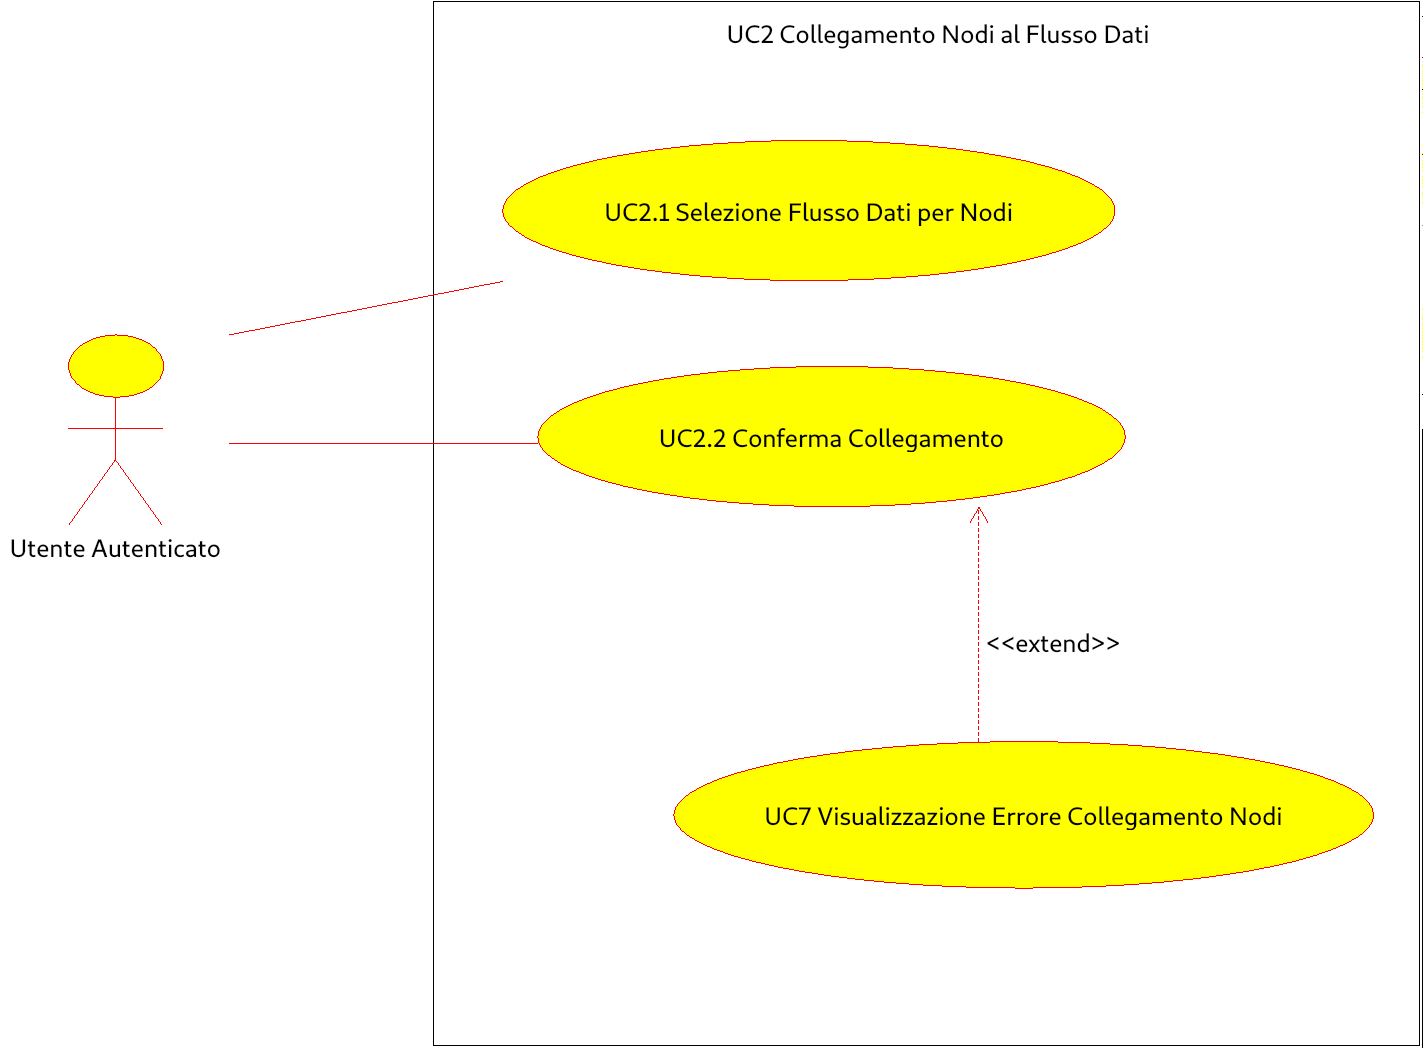
\includegraphics[scale=0.5]{./images/UC2.png}
\caption{UC2 - Collegamento nodi della rete bayesiana al flusso dati}
\end{figure}

\begin{itemize}
\item \textbf{Attore primario}: Utente;
\item \textbf{Precondizione}: l'utente ha caricato con successo la rete bayesiana (\hyperref[UC1]{UC1 (§\ref*{UC1})});
\item \textbf{Postcondizione}: L'utente ha collegato con successo i nodi desiderati della rete bayesiana caricata in \hyperref[UC1]{UC1 (§\ref*{UC1})};
\item \textbf{Scenario principale}:
	\begin{enumerate}
	\item (\hyperref[UC2.1]{UC2.1 (§\ref*{UC2.1})}) L'utente visualizza la lista di nodi che costituisce la rete bayesiana caricata in \hyperref[UC1]{UC1(§\ref*{UC1})};
	\item (\hyperref[UC2.2]{UC2.2 (§\ref*{UC2.2})}) L'utente collega i nodi desiderati ad un flusso dati;
	\item (\hyperref[UC2.3]{UC2.3 (§\ref*{UC2.3})}) L'utente conferma il collegamento dei nodi.
	\end{enumerate}
\item \textbf{Estensioni}: \hyperref[UC9]{UC9 (§\ref*{UC9})} estende \hyperref[UC2.3]{UC2.3 (§\ref*{UC2.3})}: l'utente visualizza un messaggio di errore nel caso in cui non abbia collegato alcun nodo al flusso dati.
\end{itemize}

\paragraph{UC2.1 - Visualizzazione lista di nodi della rete bayesiana e rispettivo stato}\label{UC2.1}
\begin{itemize}
\item \textbf{Attore primario:}  Utente
\item \textbf{Precondizione:} L'utente ha caricato con successo la rete bayesiana (\hyperref[UC1]{UC1 									(§\ref*{UC1})});
\item \textbf{Postcondizione:} L'utente visualizza la lista di nodi di cui la rete bayesiana è costituita, viene 			inoltre visualizzato lo stato di ogni nodo (collegato ad un flusso dati oppure no);
\item \textbf{Scenario Principale:}
	\begin{enumerate}
	\item L'ultente visualizza una lista contente i nominativi associati ad ogni nodo della rete bayesiana caricata 				in \hyperref[UC1]{UC1(§\ref*{UC1})};
	\item L'utente visualizza, accanto ai nominativi dei nodi, una lista di checkbox associate. Tali checkbox 							rappresentano lo stato del nodo a cui sono associate: "V" nel caso il nodo sia collegato ad un flusso dati, "X" 		altrimenti.
	\end{enumerate}
\end{itemize}

\paragraph{UC2.2 - Selezione flusso di dati per ogni nodo}\label{UC2.2}
\begin{itemize}
\item \textbf{Attore primario}: Utente;
\item \textbf{Precondizioni}: 
\begin{enumerate}
	\item L'utente ha caricato con successo la rete bayesiana (\hyperref[UC1]{UC1(§\ref*{UC1})});
	\item L'utente ha visualizzato la lista di nodi di cui la rete bayesiana è costituita ed il corrispondente stato 			(\hyperref[UC2.1]{UC2.1 (§\ref*{UC2.1})}).
\end{enumerate}
\item \textbf{Postcondizione}: L'utente ha collegato ogni nodo che desidera ad uno e un solo flusso dati;
\item \textbf{Scenario Principale}:
 \begin{enumerate}
 \item L'utente clicca con il cursore il nominativo corrispondente al nodo che desidera collegare ad un determinato 		flusso dati;
 \item L'utente visualizza, a seguito del click precedente, una tendina a comparsa contente i possibili flussi dati 		a cui collegare il nodo selezionato;
 \item L'utente seleziona, tramite click, il flusso dati opportuno (non sono disponibile scelte multiple) a cui 					collegare il nodo selezionato in precedenza;
 \item L'utente ripete i passaggi precedenti per ogni nodo che desidera collegare ad un flusso dati di 									monitoraggio.
 \end{enumerate}
\end{itemize}

\paragraph{UC2.3 - Conferma collegamento}\label{UC2.3}
\begin{itemize}
\item \textbf{Attore primario}: Utente;
\item \textbf{Precondizione}: L'utente ha caricato con successo la rete bayesiana (\hyperref[UC1]{UC1 (§\ref*{UC1})});
\item \textbf{Postcondizioni}: 
	\begin{enumerate}
	\item L'utente ha collegato con successo i nodi desiderati della rete bayesiana caricata in \hyperref[UC1]{UC1 				(§\ref*{UC1})} ai rispettivi flussi dati;
	\item La corrispondente checkbox di ogni nodo viene marcata con una "V" se questo è stato collegato dall'utente 				ad un flusso dati, viene invece marcata con una "X" altrimenti.
	\end{enumerate}
\item \textbf{Scenario Principale:} l'utente conferma le proprie scelte (\hyperref[UC2.2]{UC2.2 (§\ref*{UC2.2})}) cliccando il pulsante "Conferma";
\item \textbf{Estensioni}: \hyperref[UC9]{UC9 (§\ref*{UC9})}: l'utente visualizza un messaggio di errore nel caso in cui non abbia collegato alcun nodo ad un flusso dati.
\end{itemize}
\newpage

\subsubsection{UC3 - Impostazione delle politiche temporali di ricalcolo delle probabilità}\label{UC3}

\begin{figure}[H]
\centering
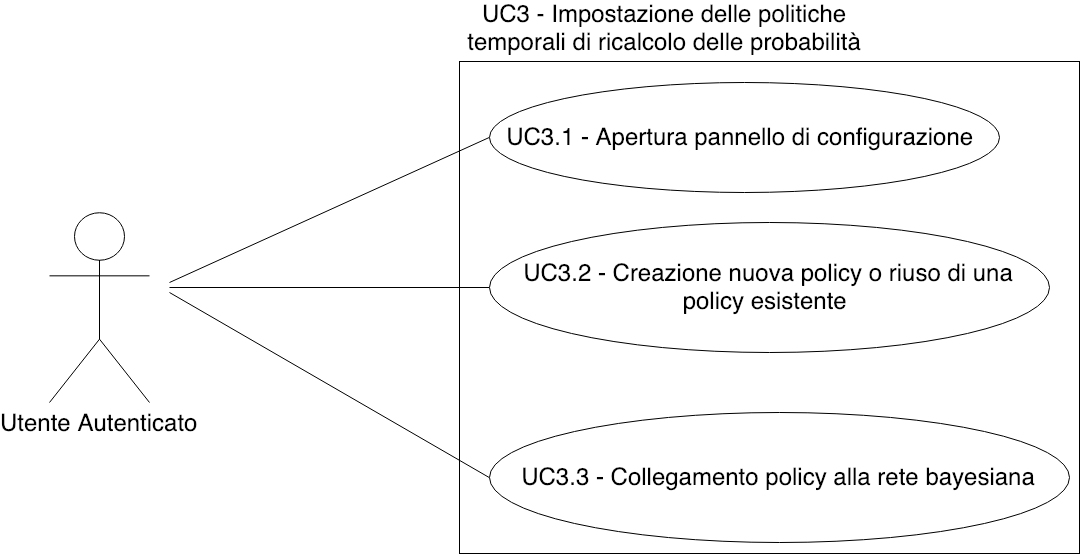
\includegraphics[scale=0.3]{./images/UC3.png}
\caption{UC3 - Impostazione delle politiche temporali di ricalcolo.}
\end{figure}

\begin{itemize}
	\item \textbf{Attore primario}: Utente; 
	\item \textbf{Precondizione}: l'utente ha caricato con successo la rete bayesiana (\hyperref[UC1]{UC1 (§\ref*{UC1})});
	\item \textbf{Postcondizione}: l'utente ha collegato con successo le policy per il ricalcolo delle probabilità alla rete bayesiana, caricata in (\hyperref[UC1]{UC1 (§\ref*{UC1})});	
	\item \textbf{Scenario Principale:}

	\begin{enumerate}
		\item L'utente accede alle impostazioni passando dalla dashboard;
		\item L'utente ha selezionato una policy esistente o ne ha creata una nuova con i parametri desiderati; 
		\item L'utente, una volta selezionata la policy, la associa  ad una rete bayesiana esistente;
		\item L'utente conferma l'associazione della policy alla rete.
	\end{enumerate}
	
\end{itemize}

\paragraph{UC3.1 - Apertura pannello di configurazione}\label{UC3.1}
\begin{itemize}
	\item \textbf{Attore primario}: Utente; 
	\item \textbf{Precondizione}: l'utente ha caricato con successo la rete bayesiana (\hyperref[UC1]{UC1 (§\ref*{UC1})});
	\item \textbf{Postcondizione}: l'utente accede al pannello di configurazione;
	\item \textbf{Scenario Principale}: l'utente, tramite un click sulla dashboard, apre il pannello di configurazione. 
\end{itemize}

\paragraph{UC3.2 - Creazione nuova policy o riuso di una policy esistente}\label{UC3.2}

\begin{itemize}
	\item \textbf{Attore primario}: Utente; 
	\item \textbf{Precondizione}: l'utente si è spostato nell'area di configurazione (\hyperref[UC3.1]{UC3.1 (§\ref*{UC3.1})});
	\item \textbf{Postcondizione}: l'utente ha selezionato la policy desiderata;
	\item \textbf{Scenario principale:}
	\begin{enumerate}
		\item L'utente dispone già di una policy e la seleziona; 
		\item L'utente crea una nuova policy, e una volta creata la seleziona. 
	\end{enumerate}
	
\end{itemize}

\paragraph{UC3.3 - Collegamento policy alla rete bayesiana}\label{UC3.3}
\begin{itemize}
	\item \textbf{Attore primario}: Utente; 
	\item \textbf{Precondizione}: l'utente ha selezionato la policy desiderata (\hyperref[UC3.2]{UC3.2 (§\ref*{UC3.2})});
	\item \textbf{Postcondizione}: l'utente ha collegato la policy selezionata ad una rete bayesiana; 
	\item \textbf{Scenario principale}: l'utente collega la policy selezionata alla rete bayesiana, impostando cosi i nuovi parametri. 
\end{itemize}

\newpage
\subsubsection{UC4 - Visualizzazione probabilità associate ai nodi non collegati al flusso}\label{UC4}

\begin{figure}[H]
\centering
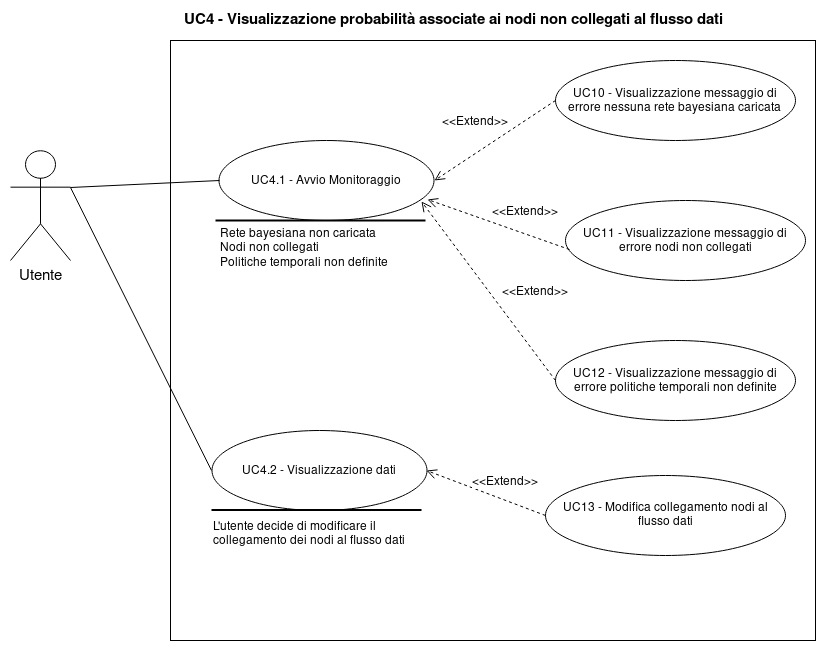
\includegraphics[scale=0.4]{./images/UC4.png}
\caption{UC4 - Visualizzazione dell probabilità associate ai nodi non collegati al flusso}
\end{figure}

\begin{itemize}
\item \textbf{Attore primario}: Utente;
\item \textbf{Precondizioni}:
	\begin{enumerate}
	\item L'utente ha collegato con successo alcuni nodi della rete bayesiana al flusso dati (\hyperref[UC2]{UC2 (§\ref*{UC2})});
	\item L'utente ha definito le politiche temporali per il ricalcolo delle probabilità relative ai nodi della rete bayesiana (\hyperref[UC3]{UC3 (§\ref*{UC3})}).
	\end{enumerate}
\item \textbf{Postcondizione}: l'utente monitora l'andamento delle probabilità dinamiche associate ad ogni nodo della rete bayesiana non collegato ad un flusso dati;
\item \textbf{Scenario Principale}: l'utente visualizza i dati forniti dai nodi della rete bayesiana, tali dati sono una misura di probabilità associata ad ogni nodo della rete bayesiana non collegato al flusso dati (\hyperref[UC2]{UC2 (§\ref*{UC2})}). Tali probabilità vengono ricalcolate,mutando dinamicamente in base alle politiche temporali stabilite in \hyperref[UC3]{UC3 (§\ref*{UC3})}.
\end{itemize}

\pagebreak

\subsubsection{UC5 - Definizione di un alert sui nodi non collegati al flusso di dati}\label{UC5}

\begin{figure}[H]
	\centering
	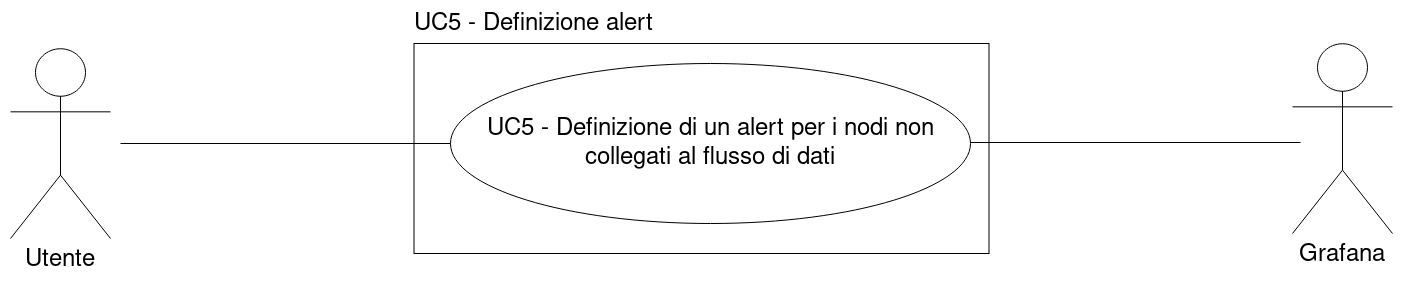
\includegraphics[scale=0.4]{./images/UC5.png}
	\caption{UC5 - Definizione di un alert sui nodi non collegati al flusso dei dati}
\end{figure}

\begin{itemize}
	\item \textbf{Attore primario}: Utente;
	\item \textbf{Attore secondario}: \textit{Grafana};
	\item \textbf{Precondizione}: alcuni nodi non sono collegati al flussi di dati;
	\item \textbf{Postcondizione}: l'utente ha aggiunto un alert per i nodi non collegati;
	\item \textbf{Scenario principale}: l'utente tramite le impostazioni di \textit{Grafana}, accessibili dai pannelli, configura l'alert desiderato.
\end{itemize}

\newpage

\subsubsection{UC6 - Rimozione di alert}\label{UC6}

\begin{figure}[H]
	\centering
	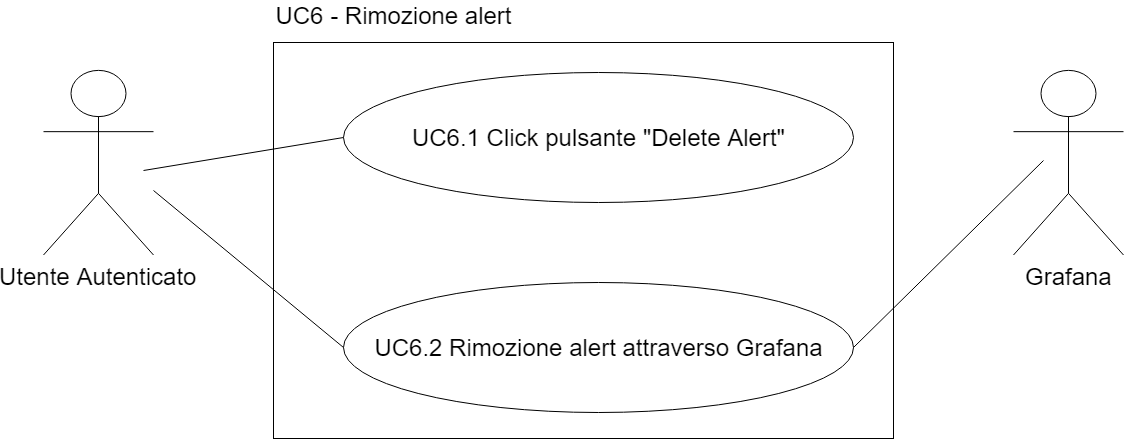
\includegraphics[scale=0.4]{./images/UC6.png}
	\caption{UC6 - Rimozione alert}
\end{figure}

\begin{itemize}
	\item \textbf{Attore primario}: Utente;
	\item \textbf{Attore secondario}: \textit{Grafana};
	\item \textbf{Precondizione:} è presente un alert associato ad un nodo non collegato ad un flusso di dati
	(\hyperref[UC5]{UC5 (§\ref*{UC5})});
	\item \textbf{Postcondizione}: l'utente ha rimosso l'alert;
	\item \textbf{Scenario principale}: l'utente rimuove l'alert desiderato, accedendo dai pannelli presenti nelle impostazioni di \textit{Grafana}.
\end{itemize}

\pagebreak

\subsubsection{UC7 - Visualizzazione alert}\label{UC7}

\begin{figure}[H]
	\centering
	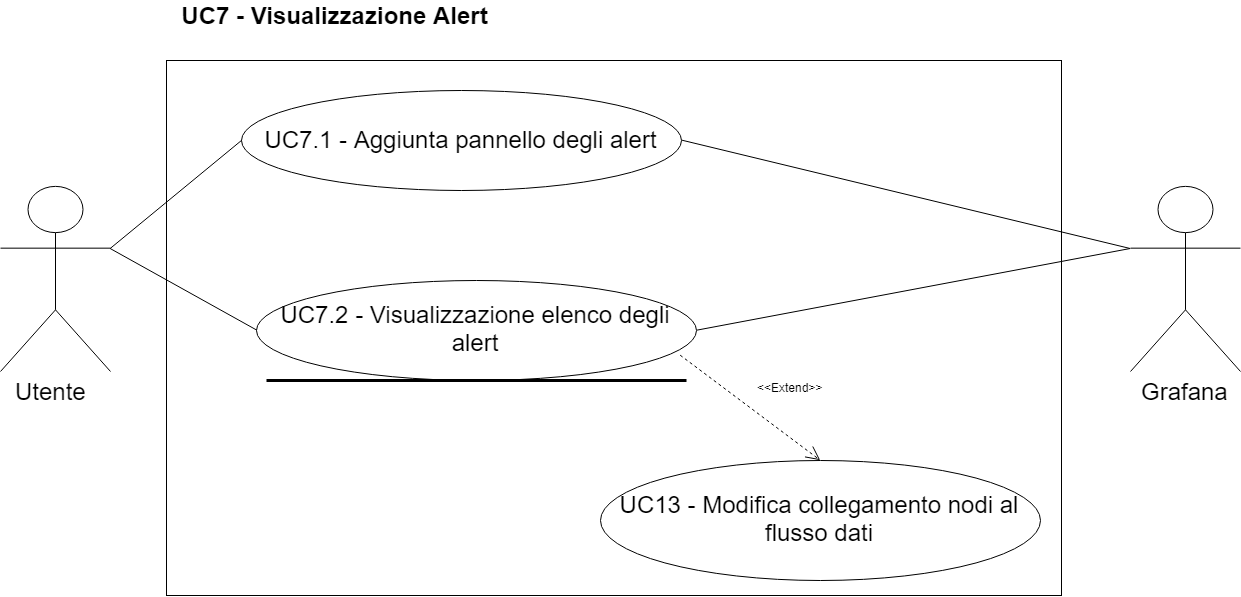
\includegraphics[scale=0.4]{./images/UC7.png}
	\caption{UC7 - Visualizzazione di un alert}
\end{figure}

\begin{itemize}
	\item \textbf{Attore primario}: Utente;
	\item \textbf{Precondizioni}: l'utente ha collegato in modo corretto i nodi 
	(\hyperref[UC2]{UC2 (§\ref*{UC2})});
	\item \textbf{Postcondizioni}: l'utente visualizza gli alert nell'apposito pannello;
	\item \textbf{Scenario principale}:
	\begin{enumerate}
		\item Il flusso di dati monitorato da \textit{Grafana} ha attivato un alert;
		\item L'utente visualizza eventuali alert derivati dai dati ottenuti da  \hyperref[UC2]{UC2 (§\ref*{UC2})}.
	\end{enumerate}
\end{itemize}

\pagebreak

\subsubsection{UC8 - Visualizzazione messaggio d'errore selezione  rete bayesiana}\label{UC8}
\begin{itemize}
\item \textbf{Attore primario}: Utente;
\item \textbf{Precondizione}: l'utente ha selezionato una rete da aggiungere ed ha cliccato il pulsante "Aggiungi", per confermare la rete. La rete selezionata dall'utente è errata per formato o per struttura;
\item \textbf{Postcondizione}: l'utente visualizza l'errore, viene quindi riportato alla finestra di selezione del file della rete baysiana (\hyperref[UC1.2]{UC1.2 (§\ref*{UC1.2})});
\item \textbf{Scenario Principale:} 
	\begin{enumerate}
		\item Viene visualizzato un messaggio d'errore che varia in base alla tipologia d'errore:
			\begin{enumerate}
				\item Estensione file della rete errato: il messaggio contiene "Il formato della rete bayesiana deve essere di tipo \textit{JSON}. Selezionare un file corretto.";
				\item Struttura errata del file: il file selezionato ha l'estensione corretta, ma il contenuto è errato. Viene visualizzato il messaggio: "La struttura della rete bayesiana selezionata non è corretta. Selezionare un file corretto.".
			\end{enumerate}
		\item L'utente clicca il pulsante con etichetta "OK".
	\end{enumerate}
\end{itemize}

\pagebreak

\subsubsection{UC9 - Visualizzazione messaggio di errore collegamento nodi}\label{UC9}
\begin{itemize}
\item \textbf{Attore primario}: Utente;
\item \textbf{Precondizione}: l'utente ha confermato il collegamento dei nodi al flusso dati (\hyperref[UC2.2]{UC2.2 (§\ref*{UC2.2})}), senza averne effettivamente collegato alcuno;
\item \textbf{Postcondizione}: l'utente visualizza l'errore;
\item \textbf{Scenario Principale}: 
	\begin{enumerate}
	\item L'utente visualizza un messaggio di errore in cui è segnalato il fatto che non sia stato collegato alcun 				nodo al flusso dati durante \hyperref[UC2]{UC2 (§\ref*{UC2})};
	\item L'utente clicca il pulsante con etichetta "OK".
	\end{enumerate}
\end{itemize}

